% Template for Cogsci submission with R Markdown

% Stuff changed from original Markdown PLOS Template
\documentclass[10pt, letterpaper]{article}

\usepackage{cogsci}
\usepackage{pslatex}
\usepackage{float}
\usepackage{caption}

% amsmath package, useful for mathematical formulas
\usepackage{amsmath}

% amssymb package, useful for mathematical symbols
\usepackage{amssymb}

% hyperref package, useful for hyperlinks
\usepackage{hyperref}

% graphicx package, useful for including eps and pdf graphics
% include graphics with the command \includegraphics
\usepackage{graphicx}

% Sweave(-like)
\usepackage{fancyvrb}
\DefineVerbatimEnvironment{Sinput}{Verbatim}{fontshape=sl}
\DefineVerbatimEnvironment{Soutput}{Verbatim}{}
\DefineVerbatimEnvironment{Scode}{Verbatim}{fontshape=sl}
\newenvironment{Schunk}{}{}
\DefineVerbatimEnvironment{Code}{Verbatim}{}
\DefineVerbatimEnvironment{CodeInput}{Verbatim}{fontshape=sl}
\DefineVerbatimEnvironment{CodeOutput}{Verbatim}{}
\newenvironment{CodeChunk}{}{}

% cite package, to clean up citations in the main text. Do not remove.
\usepackage{apacite}

% KM added 1/4/18 to allow control of blind submission


\usepackage{color}

% Use doublespacing - comment out for single spacing
%\usepackage{setspace}
%\doublespacing


% % Text layout
% \topmargin 0.0cm
% \oddsidemargin 0.5cm
% \evensidemargin 0.5cm
% \textwidth 16cm
% \textheight 21cm

\title{Information Distribution Depends on Language-Specific Features}


\author{Josef Klafka \and Daniel Yurovsky \\
        \texttt{\{jklafka, yurovsky\}@uchicago.edu} \\
       Department of Psychology \\ University of Chicago}

\begin{document}

\maketitle

\begin{abstract}
We argue for a reformulation of the Uniform Information Density
hypothesis Levy \& Jaeger (2007) in which the grammatical, phonological
and morphological features of a language determine how information is
distributed throughout utterances. We expand on a method from Yu, Cong,
Liang, \& Liu (2016) to compute entropy based on word position within
utterances as a derivation of information distribution. We analyze adult
and child spoken corpora as well as text corpora drawn from a variety of
languages on Wikipedia. We find that each language has a robust,
characteristic entropy curve across word position, and present evidence
that these entropy curves are in part determined by typological
features. We conclude that speakers may tend towards communicating
information uniformly, but the distribution of information in their
utterances is conditioned on the language they communicate in.

\textbf{Keywords:}
Entropy; information; information theory; communication
\end{abstract}

\hypertarget{introduction}{%
\section{Introduction}\label{introduction}}

Over 7,000 languages are spoken around the modern world (Simons \&
Fenning, 2018). These language vary along many dimensions, but all share
a core goal: communicating information. If speakers and writers of these
languages act near-optimally to achieve their communicative goals,
regularities of use across these diverse languages can be explained by a
rational theory of communication (Anderson, 1991). Information theory, a
mathematical framework developed by Shannon (1948) to describe the
transmission and decoding of signals, has been a unifying language for
the recent development of such theories in human and machine language
processing (Jelinek, 1976; Levy \& Jaeger, 2007).

These theories model the process of communication as transmission of
information over a noisy channel. The producer begins with an intended
meaning, packages this meaning into language, and then sends the meaning
to their intended receiver over a communcative channel. The receiver
must then decode from the signal they receive on their end of the
channel the producer's intended meaning. The problem is that the channel
is noisy, and sometimes the signal can get corrupted (e.g.~the producer
can misspeak, or the receiver can mishear). In order to maximize the
probability that the correct meaning is transmitted, these theories
predict that producers should choose linguistic messages that keep the
rate of information across words constant. The intuition is that if the
receiver misperceives a word, and that word contains most of the
information in the sentence, then the communication will have failed.
Because producers cannot predict which word a speaker will mishear,
their best strategy is spread the information evenly across all of the
words in a sentence, i.e.~maintain \emph{uniform information density}
(Genzel \& Charniak, 2002; Levy \& Jaeger, 2007).

The original evidence in Levy \& Jaeger (2007) finds that the insertion
of complementizers in relative clauses in English corresponds to where
neighboring words have high information content. Similarly, Frank \&
Jaeger (2008) argues that contradictions in English such as ``you're''
do not occur when neighboring words are highly informative. The evidence
in favor of UID largely been situation-specific and English-language
driven, while the hypothesis itself has been applied broadly over the
past decade. Applications include determining whether linguistic
alignment takes place (Jaeger \& Snider, 2013), Zipfian word length
distributions (Piantadosi, Tily, \& Gibson, 2011), communication
efficiency (Mahowald, Fedorenko, Piantadosi, \& Gibson, 2013), dialogue
and turn-taking (Xu \& Reitter, 2018) and the significance of ambiguity
in language (Piantadosi, Tily, \& Gibson, 2012), among other research.

However, other recent work has contradicted the UID hypothesis. Similar
to the original Levy \& Jaeger (2007), Zhan \& Levy (2018) focuses on
information distribution at particular points in sentences. Zhan \& Levy
(2018) finds that more information-rich classifiers in Mandarin Chinese
are produced when production of the neighboring noun is difficult, not
when the information content is high. Jain, Singh, Ranjan, Rajkumar, \&
Agarwal (2018) examine word order across spoken sentences in Hindi, a
freer word order language than English, and find that information
density has no significant effect on word order.

Recently, Yu et al. (2016) developed a more direct test of the Uniform
Information Density hypothesis, applying the logic used by Genzel \&
Charniak (2002) to look at the distribution of information \emph{within}
individual sentences. Because people process language
incrementally--using the previous words in a sentence to predict the
words that will come next--the amount of information that a word
contains when seen in isolation should increase over the course of a
sentence. Analyzing a large corpus of written English, they find a
different pattern: Entropy increases over the first few words of an
utterance and then remains constant until the final word where it again
jumps up (see Figure \ref{fig:our_replication}). Yu et al. (2016)
conclude that the Uniform Information Density hypothesis must not hold
for medial words in a sentence.

We extend and generalize Yu et al. (2016) in three ways: we confirm that
this same pattern is found in spoken English--in both adult and child
speakers. We then examine entropy curves cross-linguistically, finding a
diversity of shapes across the world's languages. Finally, we show that
entropy curves are predictable from the structure of individual
languages, namely word order. Taken together, our results suggest a
refinement of the Uniform Information Density hypothesis: speakers may
structure their utterances to optimize information density, but they
must do so under the constraints of the language they use to
communicate.

The UID hypothesis predicts that information transmission rate will tend
towards uniformity in both speech and text. We begin by examining speech
to determine if we obtain the entropy curve shape we expect for spoken
communication. We begin with the same source as Levy \& Jaeger (2007)
and Jaeger (2010), the Switchboard corpus of adult telephone
conversations. We also examine child-adult conversations in the CHILDES
TalkBank (Demuth, Culbertson, \& Alter, 2006; MacWhinney, 2014) corpora
database of spoken adult-child conversations in multiple languages.
Children are not fully developed speakers, so we want to compare the
entropy curve we obtain by computing over the utterances in the CHILDES
corpora to the utterances in the adult-adult Switchboard corpus.
Finally, we extend our cross-linguistic findings on a small number of
languages from the CHILDES experiment to a direct comparison of several
dozen languages in Wikipedia.

\hypertarget{general-methods}{%
\subsection{General methods}\label{general-methods}}

Here we will describe our adaptation of the by-word entropy method in Yu
et al. (2016), which uses the text portion of the British National
Corpus (Clear, 1993). We replicate their results at the end of this
subsection. Given a text or speech corpus divided into individual
utterances, we partition the corpus by utterance length in number of
words. For each word position \(X\) of utterances of length \(k\), we
define \(w\) as a unique word occurring in position \(X\). We further
define \(p(w)\) as the number of times word \(w\) occurs in position
\(X\), divided by the number of total words that occur in position \(X\)
i.e.~the number of sentences of length \(k\). This creates a probability
distribution over the words occurring in position \(X\), and computing
the Shannon entropy \(H(X)\) Shannon (1948) of this probability
distribution gives the positional entropy of position \(X\) in
utterances of length \(k\).

\[H(X) = \sum\limits_w p(w)\log\big(p(w)\big)\]

With this measure, we compute the unigram entropy at each position of
sentences of each length within the corpus. The result of this method
can be plotted for each utterance length as an \emph{entropy curve},
which can be visually compared across utterance length to observe the
how the unigram entropy changes across absolute positions in each of the
utterances. Genzel \& Charniak (2002) similarly examine a unigram
entropy measure on sentences, and found that entropy at the sentence
level increases linearly with sentence index within a corpus. UID
applies this uniformity of entropy rate in sentences to all levels of
speech, and so our method obtained from Yu et al. (2016), which examines
text at the word level, should find an affine function at the word
level.

The entropy curves capture individual variation across positions in
utterances of the same length. This allows us to directly observe and
judge the amount of variation in words that appear in an individual
position of a sentence. We can directly compare any two positions within
utterances to determine the amount of uncertainty, and therefore
information, on average contained by words within that position of
utterances. We are applying the same approach as in Genzel \& Charniak
(2002), but within sentences instead of across sentences.

The positional entropy at the beginning of sentences is low, then rises
and plateaus for sentence-medial word positions before dropping slightly
in the second-to-last position and rising again. However, this curve
could simply be a result of the written words in the BNC. We will expand
this analysis and replicate the result with a spoken American English
corpus.

\hypertarget{experiment-1}{%
\section{Experiment 1}\label{experiment-1}}

We replicated the Yu et al. (2016) results and found the same
characteristic three-step distribution as they did for the BNC entropy
curves.

We first used the same source for data as Levy \& Jaeger (2007), the
Switchboard corpus of American telephone conversations Godfrey,
Holliman, \& McDaniel (1992). The Switchboard corpus contains telephone
conversations of American English between strangers, with individual
utterances ranging from one word to several dozen words. We divided the
Switchboard corpus by utterance length and computed the positional
entropy for each position within each sentence length, then plotted the
result as an entropy curve.

\hypertarget{results-and-analysis}{%
\subsection{Results and Analysis}\label{results-and-analysis}}

Our plots for three representative utterance lengths are below. We found
the same characteristic shape for the American English Switchboard
corpus as in our replication of the Yu et al. (2016) results for the
BNC.

\begin{CodeChunk}
\begin{figure*}[tb]

{\centering 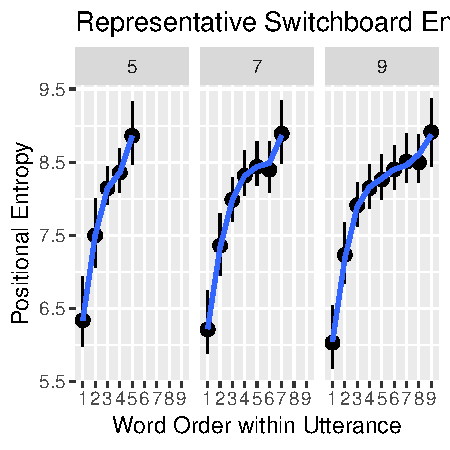
\includegraphics{figs/read_and_plot_switchboard-1} 

}

\caption[Representative Entropy Curves for the British National Corpus (top) and Switchboard (bottom)]{Representative Entropy Curves for the British National Corpus (top) and Switchboard (bottom). Points average entropies, error bars show 95\% confidence intervals computed by non-parametric bootstrap.}\label{fig:read_and_plot_switchboard}
\end{figure*}
\end{CodeChunk}

The shape we find in these two English data is notable for a number of
reasons, but what we find most interesting is one, the shape of the
distribution does not follow our predictions from UID and two, the
distribution is robust across an unrelated pair of spoken and written
English corpora. This suggests that the entropy curve is characteristic
of the English language at least, and is not a specific effect of
computing positional entropies in the written British English texts in
the BNC. For our next step, we want to expand the positional entropy
analysis to child-adult conversational corpora and languages beyond
English to see if the same three-step distribution appears.

\hypertarget{experiment-2}{%
\section{Experiment 2}\label{experiment-2}}

After replicating the Yu et al. (2016) results using the spoken
conversation corpus from Levy \& Jaeger (2007), we want to determine
whether the entropy curves will remain robust over child-adult
conversational corpora. We also wanted to see whether the curves would
show the same characteristic three-step shape across languages. To
accomplish both of these goals, we used data from the CHILDES Talkbank
system MacWhinney (2014).

The corpora in the CHILDES database consists of short and often
disconnected utterances across hours of recordings, the unigram entropy
measure is unaffected by context or lack thereof in utterances by the
adults and children in the corpora. For our first corpus, we used the
Providence English corpus Demuth et al. (2006). The Providence corpus
recorded interactions between children between 1 and 3 years old and
their parents in the home. We divided the corpus by speaker into child
and non-child categories. We further divided the corpus by utterance
length, so that all sentences of length \(k\) (e.g. \(6\)) were grouped
together. Finally, within each utterance length, we computed the unigram
entropy measure for each position. Computation of positional entropy was
identical to our general method after dividing for utterance length.

We also ran this analysis on Spanish and Mandarin corpora from CHILDES.
Spanish is an Indo-European language like English, possessing similar
grammar, word order and numerous cognate word. Mandarin Chinese is
typologically completed unrelated to English. We used the Shiro corpus
for Spanish Shiro (2000), which contains prompted narratives
individually collected from over a hundred Venezualan schoolchildren,
half from high SES backgrounds and half from low SES backgrounds. We
used the Zhou dinner corpus for Mandarin Chinese Li \& Zhou (2015),
which contains dinner conversations between 5 to 6-year-old children and
their parents collected in Shanghai.

For each corpus, we accessed transcripts of the corpus provided through
the TalkBank system and computed over the Latin alphabet transcriptions
or transliterations of the original transcriptions. For Mandarin, we
used pinyin transliterations of the utterances in the corpus with
demarcated word boundaries. The Chinese characters used for writing
Mandarin do not normally demarcate word boundaries by spacing words
apart, and for normal Chinese writing including spaces between word
boundaries can have a negative effect on reading times Bai, Yan,
Liversedge, Zang, \& Rayner (2008).

We expect that our entropy analysis on the Providence corpus will
produce an identical entropy curve shape to the BNC and Switchboard
curves. We expect similar results to English in the Spanish Shiro
entropy curve, while we expect that our Mandarin corpus will produce a
different entropy curve shape.

\hypertarget{results-and-analysis-1}{%
\subsection{Results and Analysis}\label{results-and-analysis-1}}

\begin{CodeChunk}
\begin{figure*}[tb]

{\centering 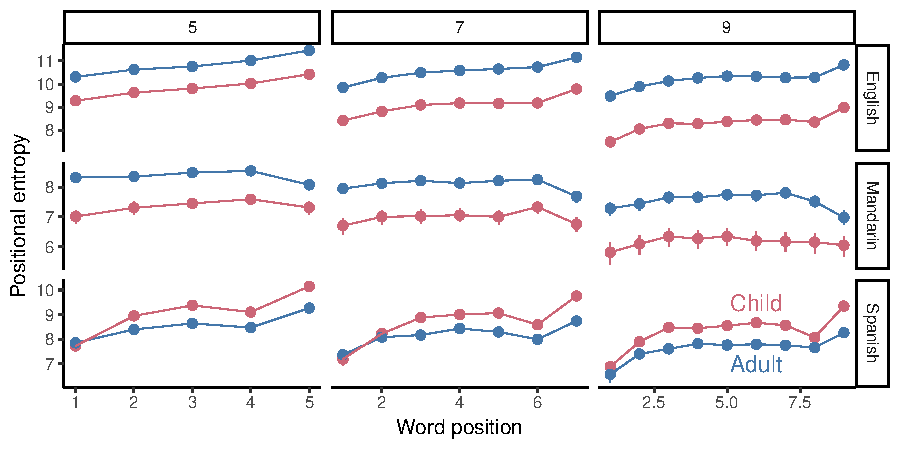
\includegraphics{figs/plot_childes-1} 

}

\caption[Representative Entropy Curves for Three Childes Corpora in English, Mandarin, and Spanish]{Representative Entropy Curves for Three Childes Corpora in English, Mandarin, and Spanish. Points average entropies, error bars show 95\% confidence intervals computed by non-parametric bootstrap.}\label{fig:plot_childes}
\end{figure*}
\end{CodeChunk}

The adult and child entropy curves track one another almost identically.
This is surprising because UID would predict that the young children in
the corpora who are not fully developed speakers would have more noise
in their distribution of information rates. This not only indicates a
robustness in the unigram entropy curve across speakers, but also across
ages and addressees. We also observed a robustness across corpora for
the same languages, and a robustness across utterance lengths within the
same corpus's entropy curve. This shows that the concept of an ``entropy
curve'' for a specific language is well-founded when considering speech
data.

We found a distinct three-step distribution for English and Spanish
CHILDES corpora, with a slight dip in the penultimate position of each
sentence. The Mandarin corpus entropy curve, by comparison, has a
noticeably lower positional entropy values in utterance-final positions
than in utterance-penultimate positions. We attribute the penultimate
dip in the English and Spanish entropy curves to the fact that most of
the utterances in the CHILDES English and Spanish corpora we examined
had a determiner such as ``the'' or ``a'' in the second-to-last position
of utterances. The beginnings of utterances in the English and Spanish
CHILDES data were usually pronouns or grammatical subjects, while the
final words were grammatical objects and had a great deal of variation
in the exact word that appeared in the utterance-final position.

These entropy curves are not what would be expected from UID. The
robustness of the three-step distribution for English and its
replication in Spanish do not resemble the affine function we would
expect from UID. The Mandarin entropy curve, which does not at all
resemble either the English/Spanish distribution or the predictions of
UID, suggests that the entropy curve can vary from language to language.
UID predicts that each language should have a similar distribution,
which should approximate an affine function.

We found that all of the English corpora followed the same three-step
entropy curve shape, regardless of whether the corpus contained spoken
or written data. The Spanish corpus we used also followed this same
shape, which we expected. However, Mandarin did not have the same shape,
indicating that the shape of the entropy curves may arise from
cross-linguistic variation. Similar grammatical and other features
between two languages, such as Spanish and English, may produce a
similar entropy curve.

\hypertarget{experiment-3}{%
\section{Experiment 3}\label{experiment-3}}

The UID hypothesis also applies to written communication: we expect
people to communicate information at a uniform rate through writing as
well. We use Wikipedia as a source for written data, which provides two
advantages. One, the quantity of data in Wikipedia is very large for
each language, at least several megabytes, and two, there are hundreds
of languages with their own Wikipedia corpora. We can therefore run our
entropy analysis on a much greater scale than using small spoken CHILDES
corpora and directly compare the results of the entropy analysis on each
language to one another. We expect to find linguistic features that
determine the shape of a language's entropy curve. We treated sentences
in the Wikipedia text corpora as equivalent to utterances in the
Switchboard and CHILDES corpora.

\hypertarget{methods}{%
\subsection{Methods}\label{methods}}

Using Giuseppe Attardi's Wikiextractor tool
\footnote{https://github.com/attardi/wikiextractor}, we extract text
corpora from Wikipedia by downloading a stored collection of Wikipedia
entries in each langauge and randomly selecting several thousand
articles from each Wikipedia language. Each language corpus was cleaned
and limited to sentences between six and \(50\) words. Similar to our
process for the Switchboard and CHILDES spoken corpora, we divided each
corpus by sentence length, and then computed our positional entropy
measure on each word position within each sentence length.

We computed two slope treatments of each curve. In the \emph{absolute}
treatment, with sentence length denoted as \(k\), we computed the slope
between positions \(1\) and \(2\), positions \(2\) and \(3\), positions
\(3\) and \(k-2\), positions \(k-2\) and \(k-1\) and positions \(k-1\)
and \(k\). For the short utterances appearing the CHILDES speech
corpora, the slopes between the first and second slopes on either end of
the distributions appeared to be more characteristic of the distribution
as a whole, with a plateau in the middle of the entropy curve for each
of the language corpora we examined in CHILDES.

However, sentences of length greater than ten in the Wikipedia corpora
were significantly more common than in the CHILDES. Therefore we also
computed relative slope treatments. In the \emph{relative 5} treatment,
we computed the slopes between every \(20\%\) of the relative word
positions in each sentence length, e.g.~the slope between \(0\%\) and
\(20\%\) of sentences of length \(10\) is the slope between the position
entropies at the sentence-initial word position and the position
representing the third word. When computing the word position index to
make those cuts, if the slope was not a whole number, then the closest
whole number position was used instead for slope calculation. Each
comparative slope within each treatment was averaged together between
different sentence lengths, for example all of the \(0\%\) to \(20\%\)
slopes over all sentence lengths were averaged together.

In both the absolute and relative \(5\) treatments, each language is
embedded in \(5\)-dimensional space. This permitted us to use cosine
similarity for direct comparison between the languages we pulled from
Wikipedia. To determine which phonological, morphological and syntactic
features affected the embedding of a language in the Wikipedia dataset,
we use the linguistic features in World Atlas of Language Structures
Dryer \& Haspelmath (2013). We checked the effects of individual
features on the embeddings of languages in the different treatments. We
computed pairwise cosine similarity between each pair of language
vectors within each treatment. For a subset of eight WALS features, we
used a generalized linear model to see whether the cosine similarity
between languages mattered in predicting if the languages shared the
same value for a WALS feature.

\hypertarget{results-and-analysis-2}{%
\subsection{Results and Analysis}\label{results-and-analysis-2}}

For eight features and \(45\) languages we pulled from Wikipedia, we
found that the cosine similarity between WALS features. The table below
shows the results for the generalized linear model we computed using
WALS features and the absolute treatment.

\begin{table}[tb]
\centering
\begin{tabular}{llrrrr}
  \hline
feature & term & estimate & std.error & statistic & p.value \\ 
  \hline
83A & cosine & 1.84 & 0.01 & 178.22 & 0.00 \\ 
  95A & cosine & 1.90 & 0.01 & 170.98 & 0.00 \\ 
  81A & cosine & 1.51 & 0.01 & 153.70 & 0.00 \\ 
  97A & cosine & 1.58 & 0.01 & 136.81 & 0.00 \\ 
  144A & cosine & 0.88 & 0.01 & 74.43 & 0.00 \\ 
  138A & cosine & 0.40 & 0.01 & 46.12 & 0.00 \\ 
  87A & cosine & 0.33 & 0.01 & 39.91 & 0.00 \\ 
  143A & cosine & 0.37 & 0.01 & 39.74 & 0.00 \\ 
  82A & cosine & 0.03 & 0.01 & 3.23 & 0.00 \\ 
   \hline
\end{tabular}
\end{table}

We also used the linear model approach to evaluate the effects of cosine
distance in the relative \(5\) treatment on the values of the same WALS
features and found similar outcomes.

From these results, we argue that cosine distance played some role in
the feature determination. The top four features in determining the WALS
feature value all characterize word order, which indicates that for this
subset of features and languages that the embeddings in the slope space
are related to the WALS features. We argue therefore that typological
features play a role in determining the positional entropy values for a
language. This indicates that the entropy curves are in some way
structured by the syntactic, morphological and phonological features of
a language.

\hypertarget{discussion}{%
\section{Discussion}\label{discussion}}

In this paper, we have extended and applied a model from Yu et al.
(2016) and derived from Genzel \& Charniak (2002) for distinguishing
entropy at each word position within sentences. We have argued that the
outcomes of this model are derived from the distribution of information
transmission in human communication. Language is not a uniform noisy
channel of communication, but each language individually represents a
different noisy channel of communication characterized in part by
typological features.

Our work complements the approach of studies such as Aylett \& Turk
(2004), where languages are characterized by a single number,
representing the rate of semantic information transfer per syllable.
This body of work attests to languages possessing different rates of
information transfer based on typological features as well. Within the
information transfer rate literature, the rate is an overall feature of
language that does not vary corpus to corpus. Similarly, in our work we
have obtained a characteristic entropy distribution for each language.
Both information rate and entropy distribution are characterized by
typological features. This indicates that the structure and rate of how
people communicate information varies cross-linguistically based on
typological features.

We initially wanted to use several hundred language corpora pulled from
Wikipedia and all \(144\) linguistic features from WALS. We considered
an computing unsupervized clusterings of the \(5\)-dimensional vectors
of our Wikipedia entropy curves, and comparing those clusterings to
clusterings of the WALS features directly using a cluster similarity
measure such as the Rand index Rand (1971). However, the problem then
arises of which combination of WALS features and how many features to
include in the clustering analysis, with \(144!\) different
combinations. Two additional problems presented themselves: one,
deciding how many clusters to use in an unsupervised clustering analysis
is an unsolved problem in machine learning; and two, not all of the
languages on Wikipedia have values inputted for their WALS features. As
a follow-up, we are considering missing-data imputation on the WALS
features in order to run the generalized linear model analysis on a
large dataset of languages.

On a more mechanical level, we expect that our entropy model will have
implications for how long people take to read individual words at
different positions of a sentence. Eye-tracking research has indicated
the effects of surprisal on fixation duration during eye-tracking
studies (Boston, Hale, Kliegl, Patil, \& Vasishth, 2008; Demberg \&
Keller, 2008; Smith \& Levy, 2013); higher surprisal of a word is on
average predictive of higher fixation duration. The \emph{wrap-up
effect} states that people process sentence-final words more slowly on
average then sentence-medial or sentence-initial words when reading, due
to integrating information to form a final understanding of the
sentence's meaning (Kuperman, Dambacher, Nuthmann, \& Kliegl, 2010;
Stowe, Kaan, Sabourin, \& Taylor, 2018). The wrap-up effect is drawn
from evidence in languages with a large final increase in their entropy
curve from our study, so we hypothesize that the supposed wrap-up effect
derives from the same source sentence-final increase in entropy curves
observed in English and other Germanic languages.

\hypertarget{acknowledgements}{%
\section{Acknowledgements}\label{acknowledgements}}

{[}Not here yet.{]}

\hypertarget{references}{%
\section{References}\label{references}}

\setlength{\parindent}{-0.1in} 
\setlength{\leftskip}{0.125in}

\noindent

\hypertarget{refs}{}
\leavevmode\hypertarget{ref-anderson1991}{}%
Anderson, J. R. (1991). The adaptive nature of human categorization.
\emph{Psychological Review}, \emph{98}(3), 409.

\leavevmode\hypertarget{ref-aylett2004}{}%
Aylett, M., \& Turk, A. (2004). The smooth signal redundancy hypothesis:
A functional explanation for relationships between redundancy, prosodic
prominence, and duration in spontaneous speech. \emph{Language and
Speech}, \emph{47}(1), 31--56.

\leavevmode\hypertarget{ref-bai2008}{}%
Bai, X., Yan, G., Liversedge, S. P., Zang, C., \& Rayner, K. (2008).
Reading spaced and unspaced chinese text: Evidence from eye movements.
\emph{Journal of Experimental Psychology: Human Perception and
Performance}, \emph{34}(5), 1277.

\leavevmode\hypertarget{ref-boston2008}{}%
Boston, M. F., Hale, J., Kliegl, R., Patil, U., \& Vasishth, S. (2008).
Parsing costs as predictors of reading difficulty: An evaluation using
the potsdam sentence corpus. \emph{Journal of Eye Movement Research},
\emph{2}(1).

\leavevmode\hypertarget{ref-clear1993}{}%
Clear, J. H. (1993). The british national corpus. \emph{The Digital
World}, 163--187.

\leavevmode\hypertarget{ref-demberg2008}{}%
Demberg, V., \& Keller, F. (2008). Data from eye-tracking corpora as
evidence for theories of syntactic processing complexity.
\emph{Cognition}, \emph{109}(2), 193--210.

\leavevmode\hypertarget{ref-demuth2006}{}%
Demuth, K., Culbertson, J., \& Alter, J. (2006). Word-minimality,
epenthesis and coda licensing in the early acquisition of english.
\emph{Language and Speech}, \emph{49}(2), 137--173.

\leavevmode\hypertarget{ref-dryer2013}{}%
Dryer, M. S., \& Haspelmath, M. (2013). \emph{The world atlas of
language structures online}. Max Planck Institute for Evolutionary
Anthropology.

\leavevmode\hypertarget{ref-frank2008}{}%
Frank, A. F., \& Jaeger, T. F. (2008). Speaking rationally: Uniform
information density as an optimal strategy for language production. In
\emph{Proceedings of the annual meeting of the cognitive science
society} (Vol. 30).

\leavevmode\hypertarget{ref-genzel2002}{}%
Genzel, D., \& Charniak, E. (2002). Entropy rate constancy in text. In
\emph{Proceedings of the 40th annual meeting on association for
computational linguistics} (pp. 199--206). Association for Computational
Linguistics.

\leavevmode\hypertarget{ref-godfrey1992}{}%
Godfrey, J. J., Holliman, E. C., \& McDaniel, J. (1992). SWITCHBOARD:
Telephone speech corpus for research and development. In
\emph{Acoustics, speech, and signal processing, 1992. ICASSP-92., 1992
ieee international conference on} (Vol. 1, pp. 517--520). IEEE.

\leavevmode\hypertarget{ref-jaeger2010}{}%
Jaeger, T. F. (2010). Redundancy and reduction: Speakers manage
syntactic information density. \emph{Cognitive Psychology},
\emph{61}(1), 23--62.

\leavevmode\hypertarget{ref-jaeger2013}{}%
Jaeger, T. F., \& Snider, N. E. (2013). Alignment as a consequence of
expectation adaptation: Syntactic priming is affected by the prime's
prediction error given both prior and recent experience.
\emph{Cognition}, \emph{127}(1), 57--83.

\leavevmode\hypertarget{ref-jain2018}{}%
Jain, A., Singh, V., Ranjan, S., Rajkumar, R., \& Agarwal, S. (2018).
Uniform information density effects on syntactic choice in hindi. In
\emph{Proceedings of the workshop on linguistic complexity and natural
language processing} (pp. 38--48).

\leavevmode\hypertarget{ref-jelinek1976}{}%
Jelinek, F. (1976). Continuous speech recognition by statistical
methods. \emph{Proceedings of the IEEE}, \emph{64}(4), 532--556.

\leavevmode\hypertarget{ref-kuperman2010}{}%
Kuperman, V., Dambacher, M., Nuthmann, A., \& Kliegl, R. (2010). The
effect of word position on eye-movements in sentence and paragraph
reading. \emph{The Quarterly Journal of Experimental Psychology},
\emph{63}(9), 1838--1857.

\leavevmode\hypertarget{ref-levy2007}{}%
Levy, R. P., \& Jaeger, T. F. (2007). Speakers optimize information
density through syntactic reduction. In \emph{Advances in neural
information processing systems} (pp. 849--856).

\leavevmode\hypertarget{ref-li2015}{}%
Li, H., \& Zhou, J. (2015). \emph{Study on dinner table talk of
preschool children family in shanghai} (Master's thesis). East China
Normal University.

\leavevmode\hypertarget{ref-macwhinney2014}{}%
MacWhinney, B. (2014). \emph{The childes project: Tools for analyzing
talk, volume ii: The database}. Psychology Press.

\leavevmode\hypertarget{ref-mahowald2013}{}%
Mahowald, K., Fedorenko, E., Piantadosi, S. T., \& Gibson, E. (2013).
Info/information theory: Speakers choose shorter words in predictive
contexts. \emph{Cognition}, \emph{126}(2), 313--318.

\leavevmode\hypertarget{ref-piantadosi2011}{}%
Piantadosi, S. T., Tily, H., \& Gibson, E. (2011). Word lengths are
optimized for efficient communication. \emph{Proceedings of the National
Academy of Sciences}, \emph{108}(9), 3526--3529.

\leavevmode\hypertarget{ref-piantadosi2012}{}%
Piantadosi, S. T., Tily, H., \& Gibson, E. (2012). The communicative
function of ambiguity in language. \emph{Cognition}, \emph{122}(3),
280--291.

\leavevmode\hypertarget{ref-rand1971}{}%
Rand, W. M. (1971). Objective criteria for the evaluation of clustering
methods. \emph{Journal of the American Statistical Association},
\emph{66}(336), 846--850.

\leavevmode\hypertarget{ref-shannon1948}{}%
Shannon, C. E. (1948). A mathematical theory of communication.
\emph{Bell System Technical Journal}, \emph{27}(3), 379--423.

\leavevmode\hypertarget{ref-shiro2000}{}%
Shiro, M. (2000). Diferencias sociales en la construcción del" yo" y
del" otro": Expresiones evaluativas en la narrativa de niños caraqueños
en edad escolar. In \emph{Lengua, discurso, texto: I simposio
internacional de análisis del discurso} (pp. 1303--1318). Visor.

\leavevmode\hypertarget{ref-simons2018}{}%
Simons, G. F., \& Fenning, C. D. (Eds.). (2018). \emph{Ethnologue:
Languages of the world, 21st edition}. Dallas, Texas: SIL International.

\leavevmode\hypertarget{ref-smith2013}{}%
Smith, N. J., \& Levy, R. (2013). The effect of word predictability on
reading time is logarithmic. \emph{Cognition}, \emph{128}(3), 302--319.

\leavevmode\hypertarget{ref-stowe2018}{}%
Stowe, L. A., Kaan, E., Sabourin, L., \& Taylor, R. C. (2018). The
sentence wrap-up dogma. \emph{Cognition}, \emph{176}, 232--247.

\leavevmode\hypertarget{ref-xu2018}{}%
Xu, Y., \& Reitter, D. (2018). Information density converges in
dialogue: Towards an information-theoretic model. \emph{Cognition},
\emph{170}, 147--163.

\leavevmode\hypertarget{ref-yu2016}{}%
Yu, S., Cong, J., Liang, J., \& Liu, H. (2016). The distribution of
information content in english sentences. \emph{arXiv Preprint
arXiv:1609.07681}.

\leavevmode\hypertarget{ref-zhan2018}{}%
Zhan, M., \& Levy, R. (2018). Comparing theories of speaker choice using
a model of classifier production in mandarin chinese. In
\emph{Proceedings of the 2018 conference of the north american chapter
of the association for computational linguistics: Human language
technologies, volume 1 (long papers)} (Vol. 1, pp. 1997--2005).

\bibliographystyle{apacite}


\end{document}
